\chapter{Choix d'implémentation}

\section{Fonctionnement général}

\paragraph{}L'utilisateur fourni un fichier et précise son type. Il peut aussi choisir d'afficher des labels sur les n\oe uds ainsi que le format de sortie souhaité. Par défaut, l'application génère un png sans labels. L'application fonctionne ensuite en trois étapes:
\begin{enumerate}
	\item Parsing du fichier d'entrée selon le type indiqué pour obtenir une représentation d'arbre selon notre structure interne.
	\item Calcul des coordonnées de chaque n\oe ud.
	\item Génération d'une image selon le type de sortie choisie.
\end{enumerate}

\begin{center}
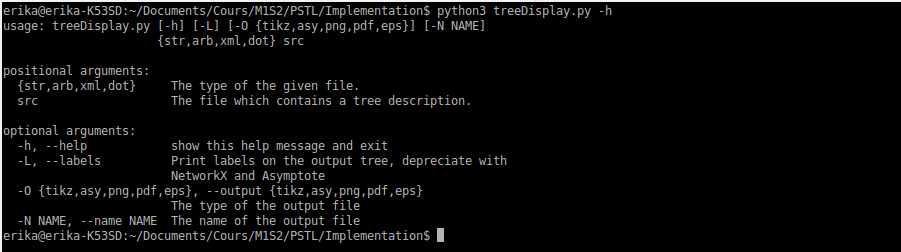
\includegraphics[width=\columnwidth]{usage}
\end{center}

\section{Plus en détails}

	\subsection{Structure d'arbre}
	
\paragraph{}Nous avons une structure d'arbre n-aire classique avec une liste pour les enfants ainsi que des attributs pour le calcul de coordonnées et la génération finale. En particulier, les attributs \verb|width| et \verb|height| représente respectivement la plus grande absisse et la plus grande ordonnée rencontrée dans le sous-arbre. Au niveau de la racine, cela représente la largeur et la hauteur du graphe.
	
\lstinputlisting[language=Python, firstline=23, lastline=37]{../Src/tree.py}

	\subsection{Fonctionnement des algorithmes de parsing}

		\subsubsection*{Mots bien parenthésés}
		
\paragraph{}Le parser de mots bien parenthésés (cf. \ref{strParser}) respecte la grammaire suivante:
		
\begin{verbatim}
ARBRE : '(' LABEL NOEUDS ')'
NOEUDS : ARBRE NOEUDS | e
LABEL : [a-zA-Z1-9]* | e
\end{verbatim}

\paragraph{} Compte-tenu du fait qu'on veut pouvoir travailler sur des arbres de grande taille, le parser bufferise le fichier d'entrée pour ne pas saturer la mémoire en chargeant tout le fichier dans une variable.

		\subsubsection*{Dot}
		
\paragraph{}Le parser dot (cf. \ref{dotParser}) parse une sous-partie du langage dot, à savoir:

\begin{verbatim}
DOT : STRICT GRAPH ID '{' SEQINST '}'
STRICT : strict | e
GRAPH = diagraph | graph
SEQINST : INST ';' SEQINST | e
INST : ID '[' label = "LABEL" ']' | ID LINK ID
LINK : -- | ->
ID : [0-9]*
LABEL : [a-zA-Z1-9]* | e
\end{verbatim}

		\subsubsection*{XML}
		
\paragraph{}Le parser XML (cf. \ref{xmlParser})respecte la grammaire ci-dessous. Comme beaucoup de langages de programmation, Python a une librairie dédiée au XML. Nous l'avons utilisée.
		
\begin{verbatim}
XML : <?xml version="1.0"?><tree> NOEUDS <tree>
NOEUDS : NOEUD NOEUDS | e
NOEUD : <node type=TAG id=ID> NOEUDS </noeud> | <leaf type=TAG id=ID />
TAG : " [a-zA-Z1-9]* "
ID : [0-9]*
\end{verbatim}

		\subsubsection*{Remarques}

\paragraph{} On veut pouvoir utiliser les fichiers générés par \verb|Arbogen| \footnote{https://github.com/fredokun/arbogen} qui est un générateur d'arbre. Il nous permet de générer des arbres de grandes tailles pour nos tests. C'est en analysant les fichiers fournis par ce générateur que nous avons établi les différences d'interprétations entre \verb|LABEL|, \verb|ID| et \verb|TAG|.

\subparagraph{}Un \verb|LABEL| est une étiquette quelconque sur un n\oe ud, qui peut apparaître à différents endroits de l'arbre. Cela nous assure qu'un mot bien parenthésés ne peut représenter qu'un arbre car seul l'arborescence des parenthèses permet de définir les arcs entre n\oe uds.

\subparagraph{}Un \verb|ID| est un identifiant unique d'un n\oe ud. On remarque alors que la grammaire Dot peut représenter des arbres mais aussi plus généralement des graphes quelconques car les \verb|ID| sont la seule façon de représenter les arcs entre n\oe uds.

\subparagraph{}Un \verb|TAG| correspond en fait à une partie gauche dans la grammaire donnée en entrée à \verb|Arbogen|. Il n'est pas donc unique dans l'arbre et est interprété dans le parser comme un label. Cependant, la grammaire XML comporte aussi des \verb|ID|. Si en plus de considérer l'arborescence des balises XML, on considérait aussi les \verb|ID|, on pourrait aussi représenter des arbres. Ce n'est pas le cas de notre parser XML car on s'intéresse aux arbres.

	\subsection{Fonctionnement de l'algorithme de calcul de coordonnées}

\paragraph{}On décide que la distance minimale entre deux n\oe uds est de $1$ unité selon l'axe des abscisses et celui des ordonnées.

\paragraph{}L'ordonnée d'un n\oe ud est triviale: c'est sa profondeur.

\paragraph{}L'abcisse d'un n\oe ud est un peu plus complexe et demande donc plus de réflexion. 

\subparagraph{}On veut qu'un père soit centré sur ses fils. On commence donc par placer ses fils s'il en a puis on fait la moyenne de l'abscisse de ses $2$ fils extrémaux pour le centrer. 

\subparagraph{}Si un n\oe ud n'a pas de fils, on le place à $1$ de son frère gauche. D'un point de vue de l'architecture, on a donc besoin d'une structure qui, à profondeur \verb|p| mémorise la prochaine place disponible (ou au choix la dernière place utilisée).

\subparagraph{}Si un n\oe ud a des fils, il se peut qu'en calculant son abscisse en fonction de ses fils on se retrouve avec un n\oe ud qui est trop proche de son frère gauche comme dans l'exemple ci-dessous. 

\subparagraph{} Considérons l'arbre suivant: \verb|(root (n11) (n12) (n13 (n21) (n22) (n23)))|. \\
\begin{tabular}{|l|c|c|c|c|c|c|c|c|c|c|c|c|c|c|}
	\hline
	 & \multicolumn{2}{|c|}{root} & \multicolumn{2}{|c|}{n11} & \multicolumn{2}{|c|}{n12} & \multicolumn{2}{|c|}{n13} & \multicolumn{2}{|c|}{n21} & \multicolumn{2}{|c|}{n22} & \multicolumn{2}{|c|}{n23}\\ \hline
	& x & y & x & y & x & y & x & y & x & y & x & y & x & y \\ \hline
	Inititalement & -1 & 0 & -1 & 0 & -1 & 0 & -1 & 0 & -1 & 0 & -1 & 0 & -1 & 0 \\ \hline
	Appel sur root & -1 & 0 & -1 & 0 & -1 & 0 & -1 & 0 & -1 & 0 & -1 & 0 & -1 & 0 \\ \hline
	Appel sur n11 & -1 & 0 & 0 & 1 & -1 & 0 & -1 & 0 & -1 & 0 & -1 & 0 & -1 & 0 \\ \hline
	Retour sur root & -1 & 0 & 0 & 1 & -1 & 0 & -1 & 0 & -1 & 0 & -1 & 0 & -1 & 0 \\ \hline
	Appel sur n12 & -1 & 0 & 0 & 1 & 1 & 1 & -1 & 0 & -1 & 0 & -1 & 0 & -1 & 0 \\ \hline
	Retour sur root & -1 & 0 & 0 & 1 & 1 & 1 & -1 & 0 & -1 & 0 & -1 & 0 & -1 & 0 \\ \hline
	Appel sur n13 & -1 & 0 & 0 & 1 & 1 & 1 & -1 & 0 & -1 & 0 & -1 & 0 & -1 & 0 \\ \hline
	Appel sur n21 & -1 & 0 & 0 & 1 & 1 & 1 & -1 & 0 & 0 & 2 & -1 & 0 & -1 & 0 \\ \hline
	Retour sur n13 & -1 & 0 & 0 & 1 & 1 & 1 & -1 & 0 & 0 & 2 & -1 & 0 & -1 & 0 \\ \hline
	Appel sur n22 & -1 & 0 & 0 & 1 & 1 & 1 & -1 & 0 & 0 & 2 & 1 & 2 & -1 & 0 \\ \hline
	Retour sur n13 & -1 & 0 & 0 & 1 & 1 & 1 & -1 & 0 & 0 & 2 & 1 & 2 & -1 & 0 \\ \hline
	Appel sur n23 & -1 & 0 & 0 & 1 & 1 & 1 & -1 & 0 & 0 & 2 & 1 & 2 & 2 & 2 \\ \hline
	Retour sur n13 & -1 & 0 & 0 & 1 & 1 & 1 & -1 & 0 & 0 & 2 & 1 & 2 & 2 & 2 \\ \hline
\end{tabular}\\
La position ensuite calculée pour \verb|n13| est $1$. Or il y a déjà \verb|n12| à cet endroit. La première place disponible à profondeur $1$ est $2$. On va donc devoir effectuer un décalage de $1$.

\begin{figure}[h] \centering \resizebox {!}{4cm} {
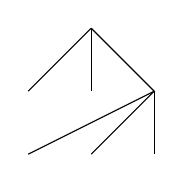
\begin{tikzpicture}[scale=0.8, every node/.style={scale=0.8}, node distance=1pt]
\draw (1.000000, -0.000000) -- (0.000000, -1.000000);
\draw (1.000000, -0.000000) -- (1.000000, -1.000000);
\draw (2.000000, -1.000000) -- (0.000000, -2.000000);
\draw (2.000000, -1.000000) -- (1.000000, -2.000000);
\draw (2.000000, -1.000000) -- (2.000000, -2.000000);
\draw (1.000000, -0.000000) -- (2.000000, -1.000000);

\end{tikzpicture}}
\caption{Résultat de l'exemple à la fin de l'étape 1.}
\end{figure}

\subparagraph{}On compare la position calculée avec la première position disponible et on prend le max. Si la position calculée n'est pas celle retenue, le père n'est plus centré au milieu de ses fils. On mémorise donc le décalage effectué pour ce père pour ensuite l'appliquer à ses sous-arbres dans un second temps pour des raisons de complexité. En effet, si on faisait chaque décalage lorsqu'il se présentait, le décalage serait quadratique car il y a potentiellement un décalage pour chaque ancêtre d'un n\oe uds.
	
\lstinputlisting[language=Python, firstline=43, lastline=72]{../Src/tree.py}

\subparagraph{}Il faut ensuite appliquer récursivement les décalages calculés lors de la première passe. On calcule à la même occasion la hauteur et la largeur de l'image pour pouvoir connaître le ratio de l'image lors de la génération.

\lstinputlisting[language=Python, firstline=77, lastline=87]{../Src/tree.py}

\subparagraph{}Le résultat finale est le suivant:

\begin{figure}[h] \centering \resizebox {!}{5cm} {
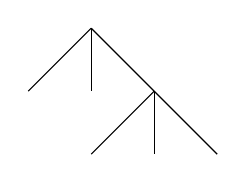
\begin{tikzpicture}[scale=0.8, every node/.style={scale=0.8}, node distance=1pt]
\draw (1.000000, -0.000000) -- (0.000000, -1.000000);
\draw (1.000000, -0.000000) -- (1.000000, -1.000000);
\draw (2.000000, -1.000000) -- (1.000000, -2.000000);
\draw (2.000000, -1.000000) -- (2.000000, -2.000000);
\draw (2.000000, -1.000000) -- (3.000000, -2.000000);
\draw (1.000000, -0.000000) -- (2.000000, -1.000000);

\end{tikzpicture}}
\caption{Résultat de l'exemple à la fin de l'étape 2.}
\end{figure}

	\subsection{Fonctionnement de la génération du code}
	
		\subsubsection*{TikZ}
\lstinputlisting[language=Python, firstline=20]{../Src/toTikZ.py}
		
		\subsubsection*{Asymptote}
\lstinputlisting[language=Python, firstline=20]{../Src/toAsymptote.py}
		
		\subsubsection*{Autre}
\lstinputlisting[language=Python, firstline=20]{../Src/toNetworkX.py}

\section{Complexité}

\paragraph{}On suppose que la taille des labels est bornée. On note $n$ le nombre de n\oe uds dans l'arbre. Dans ce cas:

\begin{enumerate}
	\item Le parsing d'un fichier est en $O(n)$ car on parcours linéairement le fichier.
	\item Le calcul des coordonnées est en $O(n)$ car on effectue $2$ passes sur l'arbre et lors de chaque passe on visite une et une seule fois chaque n\oe ud.
	\item La génération du fichier de sortie est en $O(n)$ car on visite une unique fois chaque n\oe ud pour écrire ses coordonnées dans le fichier de sortie.
\end{enumerate}
On a donc une complexité générale en $O(n)$ où $n$ est le nombre de n\oe ud de l'arbre.

\paragraph{}Notons que nous avons supposé que la taille des labels était bornée. Or nous n'avons aucune prise sur la taille des labels du fichier qui nous est passé en entrée. Dans ce cas, même si on borne la taille des labels pour l'affichage, la complexité est dominée par le parsing du fichier d'entrée car on doit lire tous les caractères du fichier.